\documentclass[11pt,compress,t,notes=noshow, xcolor=table]{beamer}
\usepackage[]{graphicx}\usepackage[]{color}
% maxwidth is the original width if it is less than linewidth
% otherwise use linewidth (to make sure the graphics do not exceed the margin)
\makeatletter
\def\maxwidth{ %
  \ifdim\Gin@nat@width>\linewidth
    \linewidth
  \else
    \Gin@nat@width
  \fi
}
\makeatother

\newcommand{\citebutton}[2]{%
\beamergotobutton{\href{#2}{#1}}%
}

\newcommand{\blu}[1]{\textcolor{blue}{#1}}
\newcommand{\org}[1]{\textcolor{orange}{#1}}
\newcommand{\ques}{\textbf{\textcolor{red}{Question:  }}}
\newcommand{\questionssofar}{\begin{frame}\frametitle{Any questions?}\end{frame}}

\newcommand\warning{%
 \makebox[1.4em][c]{%
 \makebox[0pt][c]{\raisebox{.1em}{\scriptsize!}}%
 \makebox[0pt][c]{\color{red}\normalsize$\bigtriangleup$}}}%

\definecolor{fgcolor}{rgb}{0.345, 0.345, 0.345}
\newcommand{\hlnum}[1]{\textcolor[rgb]{0.686,0.059,0.569}{#1}}%
\newcommand{\hlstr}[1]{\textcolor[rgb]{0.192,0.494,0.8}{#1}}%
\newcommand{\hlcom}[1]{\textcolor[rgb]{0.678,0.584,0.686}{\textit{#1}}}%
\newcommand{\hlopt}[1]{\textcolor[rgb]{0,0,0}{#1}}%
\newcommand{\hlstd}[1]{\textcolor[rgb]{0.345,0.345,0.345}{#1}}%
\newcommand{\hlkwa}[1]{\textcolor[rgb]{0.161,0.373,0.58}{\textbf{#1}}}%
\newcommand{\hlkwb}[1]{\textcolor[rgb]{0.69,0.353,0.396}{#1}}%
\newcommand{\hlkwc}[1]{\textcolor[rgb]{0.333,0.667,0.333}{#1}}%
\newcommand{\hlkwd}[1]{\textcolor[rgb]{0.737,0.353,0.396}{\textbf{#1}}}%
\let\hlipl\hlkwb

\usepackage{framed}
\makeatletter
\newenvironment{kframe}{%
 \def\at@end@of@kframe{}%
 \ifinner\ifhmode%
  \def\at@end@of@kframe{\end{minipage}}%
  \begin{minipage}{\columnwidth}%
 \fi\fi%
 \def\FrameCommand##1{\hskip\@totalleftmargin \hskip-\fboxsep
 \colorbox{shadecolor}{##1}\hskip-\fboxsep
     % There is no \\@totalrightmargin, so:
     \hskip-\linewidth \hskip-\@totalleftmargin \hskip\columnwidth}%
 \MakeFramed {\advance\hsize-\width
   \@totalleftmargin\z@ \linewidth\hsize
   \@setminipage}}%
 {\par\unskip\endMakeFramed%
 \at@end@of@kframe}
\makeatother

\definecolor{shadecolor}{rgb}{.97, .97, .97}
\definecolor{messagecolor}{rgb}{0, 0, 0}
\definecolor{warningcolor}{rgb}{1, 0, 1}
\definecolor{errorcolor}{rgb}{1, 0, 0}
\newenvironment{knitrout}{}{} % an empty environment to be redefined in TeX

\usepackage{alltt}
\newcommand{\SweaveOpts}[1]{}  % do not interfere with LaTeX
\newcommand{\SweaveInput}[1]{} % because they are not real TeX commands
\newcommand{\Sexpr}[1]{}       % will only be parsed by R
\newcommand{\xmark}{\ding{55}}%


\usepackage[english]{babel}
\usepackage[utf8]{inputenc}

\usepackage{dsfont}
\usepackage{verbatim}
\usepackage{amsmath}
\usepackage{amsfonts}
\usepackage{amssymb}
\usepackage{bm}
\usepackage{csquotes}
\usepackage{multirow}
\usepackage{longtable}
\usepackage{booktabs}
\usepackage{enumerate}
\usepackage[absolute,overlay]{textpos}
\usepackage{psfrag}
\usepackage{algorithm}
\usepackage{algpseudocode}
\usepackage{eqnarray}
\usepackage{arydshln}
\usepackage{tabularx}
\usepackage{placeins}
\usepackage{tikz}
\usepackage{setspace}
\usepackage{colortbl}
\usepackage{mathtools}
\usepackage{wrapfig}
\usepackage{bm}
\usepackage{amsmath}
\usepackage{pifont}

\usetikzlibrary{shapes.multipart,shapes,arrows,automata,positioning,calc,chains,trees, shadows}
\tikzset{
  %Define standard arrow tip
  >=stealth',
  %Define style for boxes
  punkt/.style={
    rectangle,
    rounded corners,
    draw=black, very thick,
    text width=6.5em,
    minimum height=2em,
    text centered},
  % Define arrow style
  pil/.style={
    ->,
    thick,
    shorten <=2pt,
    shorten >=2pt,}
}

\tikzstyle{vec}=[draw, rectangle, fill = white, minimum width=5mm, minimum height=1cm, inner sep = 2pt]

\usepackage{subfig}

% Defines macros and environments
\usepackage{../../style/lmu-lecture}


\let\code=\texttt
\let\proglang=\textsf

\setkeys{Gin}{width=0.9\textwidth}

\setbeamertemplate{frametitle}{\expandafter\uppercase\expandafter\insertframetitle}

\usepackage{bbm}
% basic latex stuff
\newcommand{\pkg}[1]{{\fontseries{b}\selectfont #1}} %fontstyle for R packages
\newcommand{\lz}{\vspace{0.5cm}} %vertical space
\newcommand{\dlz}{\vspace{1cm}} %double vertical space
\newcommand{\oneliner}[1] % Oneliner for important statements
{\begin{block}{}\begin{center}\begin{Large}#1\end{Large}\end{center}\end{block}}


%new environments
\newenvironment{vbframe}  %frame with breaks and verbatim
{
 \begin{frame}[containsverbatim,allowframebreaks]
}
{
\end{frame}
}

\newenvironment{vframe}  %frame with verbatim without breaks (to avoid numbering one slided frames)
{
 \begin{frame}[containsverbatim]
}
{
\end{frame}
}

\newenvironment{blocki}[1]   % itemize block
{
 \begin{block}{#1}\begin{itemize}
}
{
\end{itemize}\end{block}
}

\newenvironment{fragileframe}[2]{  %fragile frame with framebreaks
\begin{frame}[allowframebreaks, fragile, environment = fragileframe]
\frametitle{#1}
#2}
{\end{frame}}


\newcommand{\myframe}[2]{  %short for frame with framebreaks
\begin{frame}[allowframebreaks]
\frametitle{#1}
#2
\end{frame}}

\newcommand{\remark}[1]{
  \textbf{Remark:} #1
}


\newenvironment{deleteframe}
{
\begingroup
\usebackgroundtemplate{
\includegraphics[width=\paperwidth,height=\paperheight]{../style/color/red.png}}
 \begin{frame}
}
{
\end{frame}
\endgroup
}
\newenvironment{simplifyframe}
{
\begingroup
\usebackgroundtemplate{
\includegraphics[width=\paperwidth,height=\paperheight]{../style/color/yellow.png}}
 \begin{frame}
}
{
\end{frame}
\endgroup
}\newenvironment{draftframe}
{
\begingroup
\usebackgroundtemplate{
\includegraphics[width=\paperwidth,height=\paperheight]{../style/color/green.jpg}}
 \begin{frame}
}
{
\end{frame}
\endgroup
}
% https://tex.stackexchange.com/a/261480: textcolor that works in mathmode
\makeatletter
\renewcommand*{\@textcolor}[3]{%
  \protect\leavevmode
  \begingroup
    \color#1{#2}#3%
  \endgroup
}
\makeatother





\input{../../latex-math/basic-math.tex}
\input{../../latex-math/basic-ml.tex}

%\newcommand{\titlefigure}{figure/gpt_sq.png}
\newcommand{\learninggoals}{
\item illustrate chain-of-thought and point out the benefits it brings to LLMs
\item illustrate tree-of-thought and point out the benefits it brings to LLMs 
}

\definecolor{texblue}{rgb}{0, 0, 1}
\def\myblue#1{\textcolor{texblue}{#1}}

\title{Chain-of-thought Prompting}
% \author{}
\institute{\href{https://slds-lmu.github.io/lecture_dl4nlp/}{slds-lmu.github.io/lecture\_dl4nlp}}
\date{}

\begin{document}
\lecturechapter{Large Language Models (LLMs)}
\lecture{Deep Learning for NLP}

% ------------------------------------------------------------------------------ 

\begin{vbframe}{chain-of-though motivation}

\vfill

How to boost the reasoning capabilities of LLMs? \citebutton{Wei et al., 2021}{https://arxiv.org/abs/2109.01652}

\begin{itemize}
\item Training or tuning with formal languages works well
    \begin{itemize}
    \item Still, templates \& labeled data are costly to create
    \end{itemize}
\item Few-shot learning via prompting works for most tasks
    \begin{itemize}
    \item Still, it works poorly on tasks that require reasoning
    \end{itemize}
\item Chain of thought (CoT) prompting
    \begin{itemize}
    \item Prompts in the form <input, \textit{chain of thought}, output>
    \item CoT: series of intermediate steps that lead to a final output
    \end{itemize}

\end{itemize}

\vfill

\end{vbframe}

% ------------------------------------------------------------------------------ 

\begin{vbframe}{Chain-of-thought prompting paradigm}

\vfill

\textbf{CoT enables LLMs to tackle complex arithmetic, commonsense, and symbolic reasoning tasks.}

\begin{figure}
    \centering
    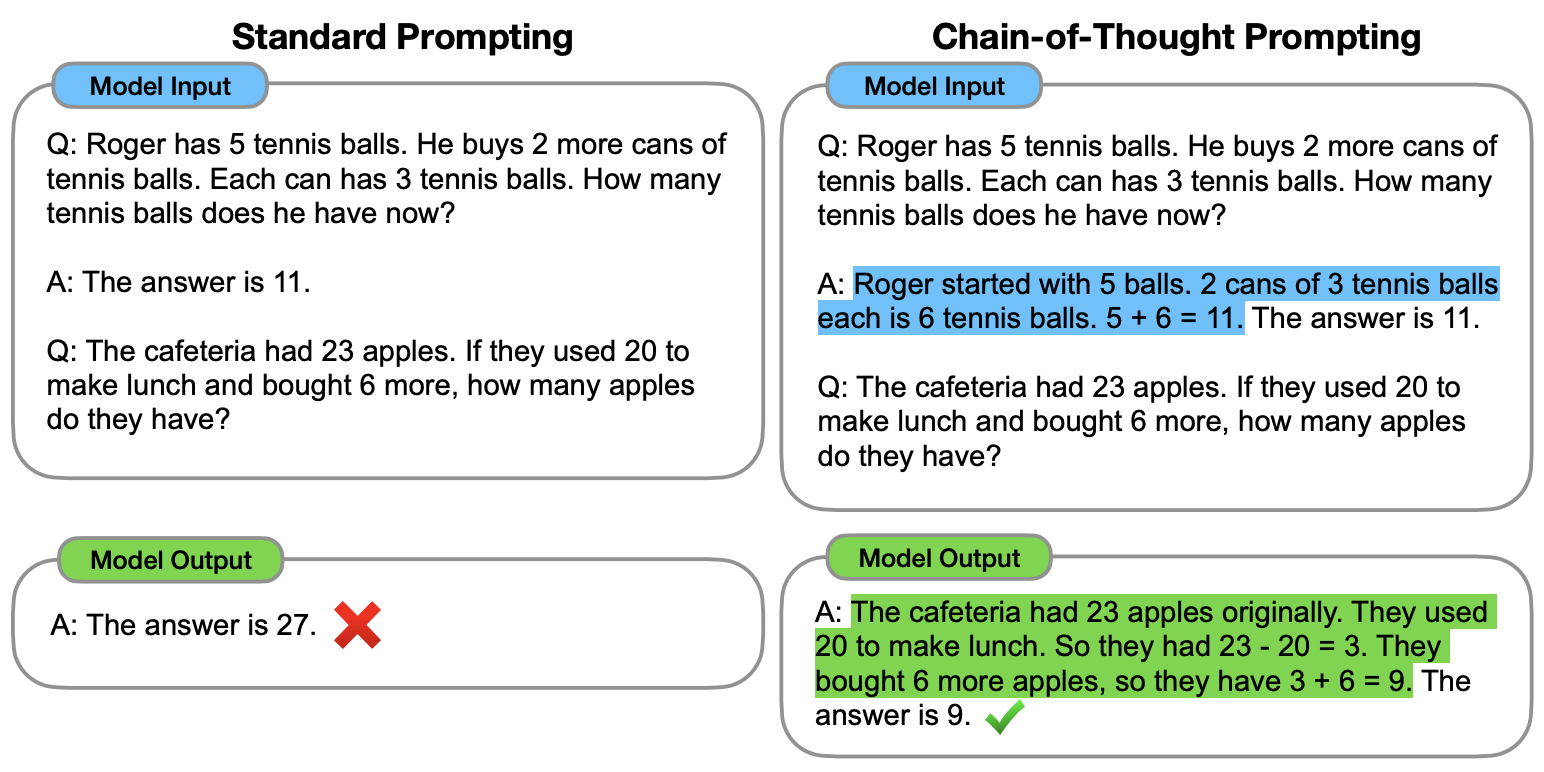
\includegraphics{figure/chain_of_thought.png}\\
    \citebutton{Source: Wei et al., 2022}{https://arxiv.org/pdf/2201.11903.pdf}
\end{figure}

\vfill

\end{vbframe}

% ------------------------------------------------------------------------------


\begin{vbframe}{Benefits of Chain-of-thought}

\vfill

\begin{itemize}
    \item Decompose multi-step problems and thus allocate more compute to problems requiring more reasoning steps
    \item By describing the reasoning, interpretability is increased. It provides the possibility to observe where reasoning went wrong
    \item It is closer to how humans solve tasks using language
    \item By designing a prompt, existing large language models are able to perform chain-of-thought reasoning.
\end{itemize}

\vfill

\end{vbframe}


% ------------------------------------------------------------------------------

\begin{vbframe}{Examples (1)}

\vfill

\textbf{Examples of $<$input, chain of thought, output$>$ triples for arithmetic, commonsense, and symbolic reasoning}

\begin{figure}
    \centering
    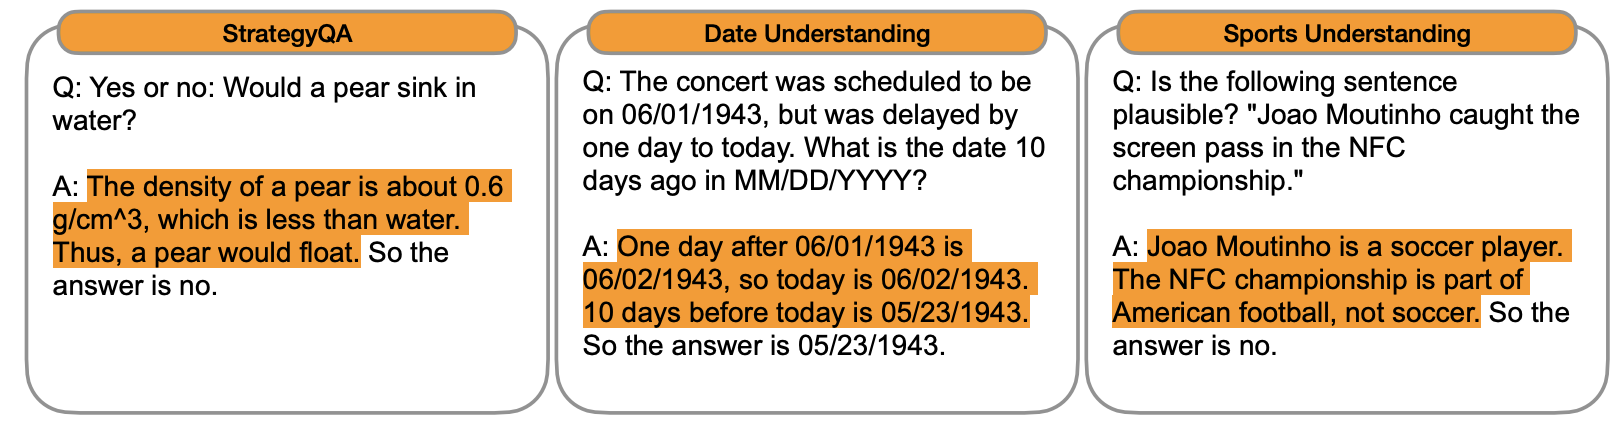
\includegraphics{figure/cot_examples_1.png}\\
    \citebutton{Source: Wei et al., 2022}{https://arxiv.org/pdf/2201.11903.pdf}
\end{figure}

\vfill

\end{vbframe}

% ------------------------------------------------------------------------------

\begin{vbframe}{Examples (2)}

\vfill

\textbf{Examples of $<$input, chain of thought, output$>$ triples for arithmetic, commonsense, and symbolic reasoning}

\begin{figure}
    \centering
    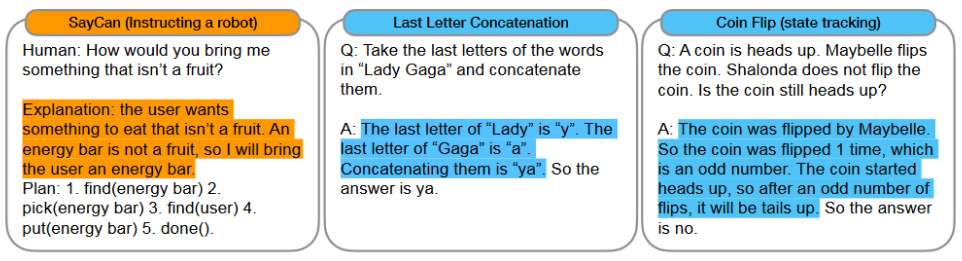
\includegraphics{figure/cot_examples_2.png}\\
    \citebutton{Source: Wei et al., 2022}{https://arxiv.org/pdf/2201.11903.pdf}
\end{figure}

\vfill

\end{vbframe}

% ------------------------------------------------------------------------------

\begin{vbframe}{CoT improves arithmetics}

%\vfill

SVAMP: math word problems with varying structures; MAWPS:
repository unifying math problems from different sources;
    \citebutton{Source: Wei et al., 2022}{https://arxiv.org/pdf/2201.11903.pdf}

\begin{figure}
    \centering
    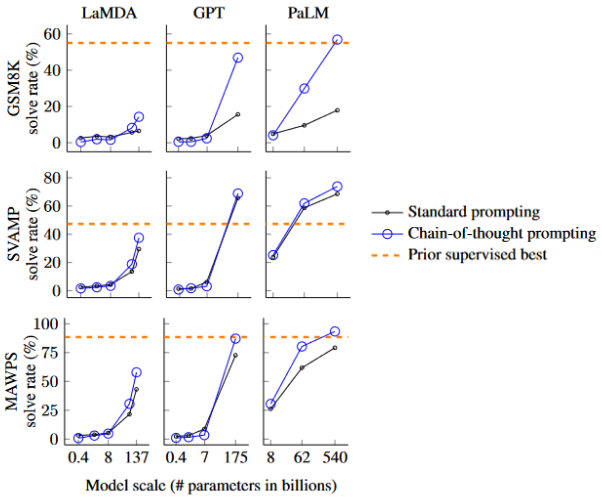
\includegraphics[width=0.5\textwidth]{figure/cot_performance1.png}
\end{figure}

%\vfill

\end{vbframe}

% ------------------------------------------------------------------------------

\begin{vbframe}{CoT improves commonsense}

\vfill

CSQA: Contains around 200K dialogs with a total of 1.6M
turns. Further, unlike existing large scale QA datasets
which contain simple questions that can be answered from a
single tuple, the questions in the dialogs require a larger
subgraph of the KG. 


\begin{figure}
    \centering
    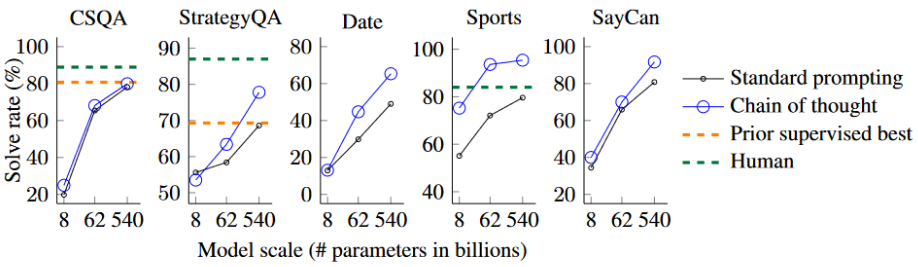
\includegraphics{figure/cot_performance2.png}\\
    \citebutton{Source: Wei et al., 2022}{https://arxiv.org/pdf/2201.11903.pdf}
\end{figure}

\vfill

\end{vbframe}

% ------------------------------------------------------------------------------ 

\begin{vbframe}{tree-of-thought: motivation}

\vfill

\begin{itemize}
\item The token-level and left-to-right decisions of the autoregressive mechanism pose a limitation for:
    \begin{itemize}
    \item Tasks where initial decisions play a pivotal role
    \item Tasks requiring exploration or strategic lookahead
    \end{itemize}
\item Potential strategy to solve those:
    \begin{itemize}
    \item Maintain and explore diverse alternatives instead of just picking one
    \item Evaluates current status and looks ahead or backtrack to make global decisions
    \end{itemize}

\end{itemize}

\vfill

\end{vbframe}

% ------------------------------------------------------------------------------

\begin{vbframe}{Tree-of-thought: prompting paradigm}

\vfill

Schematic illustrating various approaches to problem solving with LLMs. Each rectangle box represents a \textit{thought}, a coherent language sequence serving as an intermediate step toward problem solving.

\begin{figure}
    \centering
    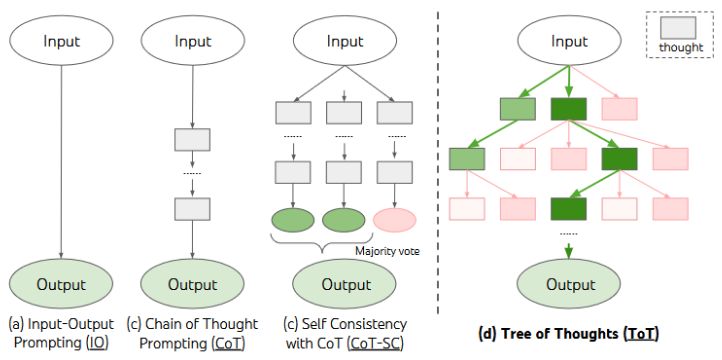
\includegraphics{figure/tot_vs_cot.png}\\
\citebutton{Yao et al., 2023}{https://arxiv.org/pdf/2305.10601.pdf}
\end{figure}

\vfill

\end{vbframe}

% ------------------------------------------------------------------------------


\begin{vbframe}{Tree-of-thought for creative writing}

\vfill

A step of deliberate search in a randomly picked Creative Writing task. Given the input, the LM samples five different plans, and then votes five times to decide which plan is best.
    
\begin{figure}
    \centering
    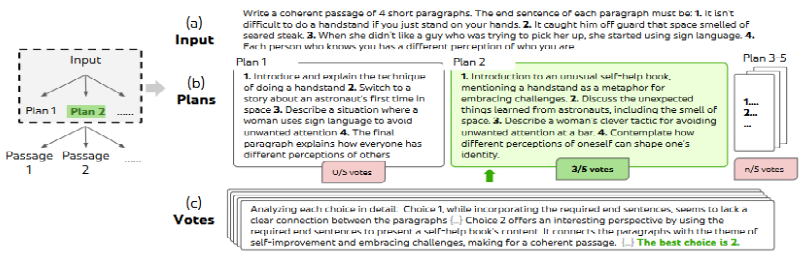
\includegraphics{figure/tot_creative_writing.png}\\
\citebutton{Yao et al., 2023}{https://arxiv.org/pdf/2305.10601.pdf}
\end{figure}

\vfill

\end{vbframe}

\begin{vbframe}{Tree-of-thought for creative writing (2)}

\vfill
    
\begin{figure}
    \raisebox{0pt}[\height][\depth]{\hspace{-0.85cm}%
        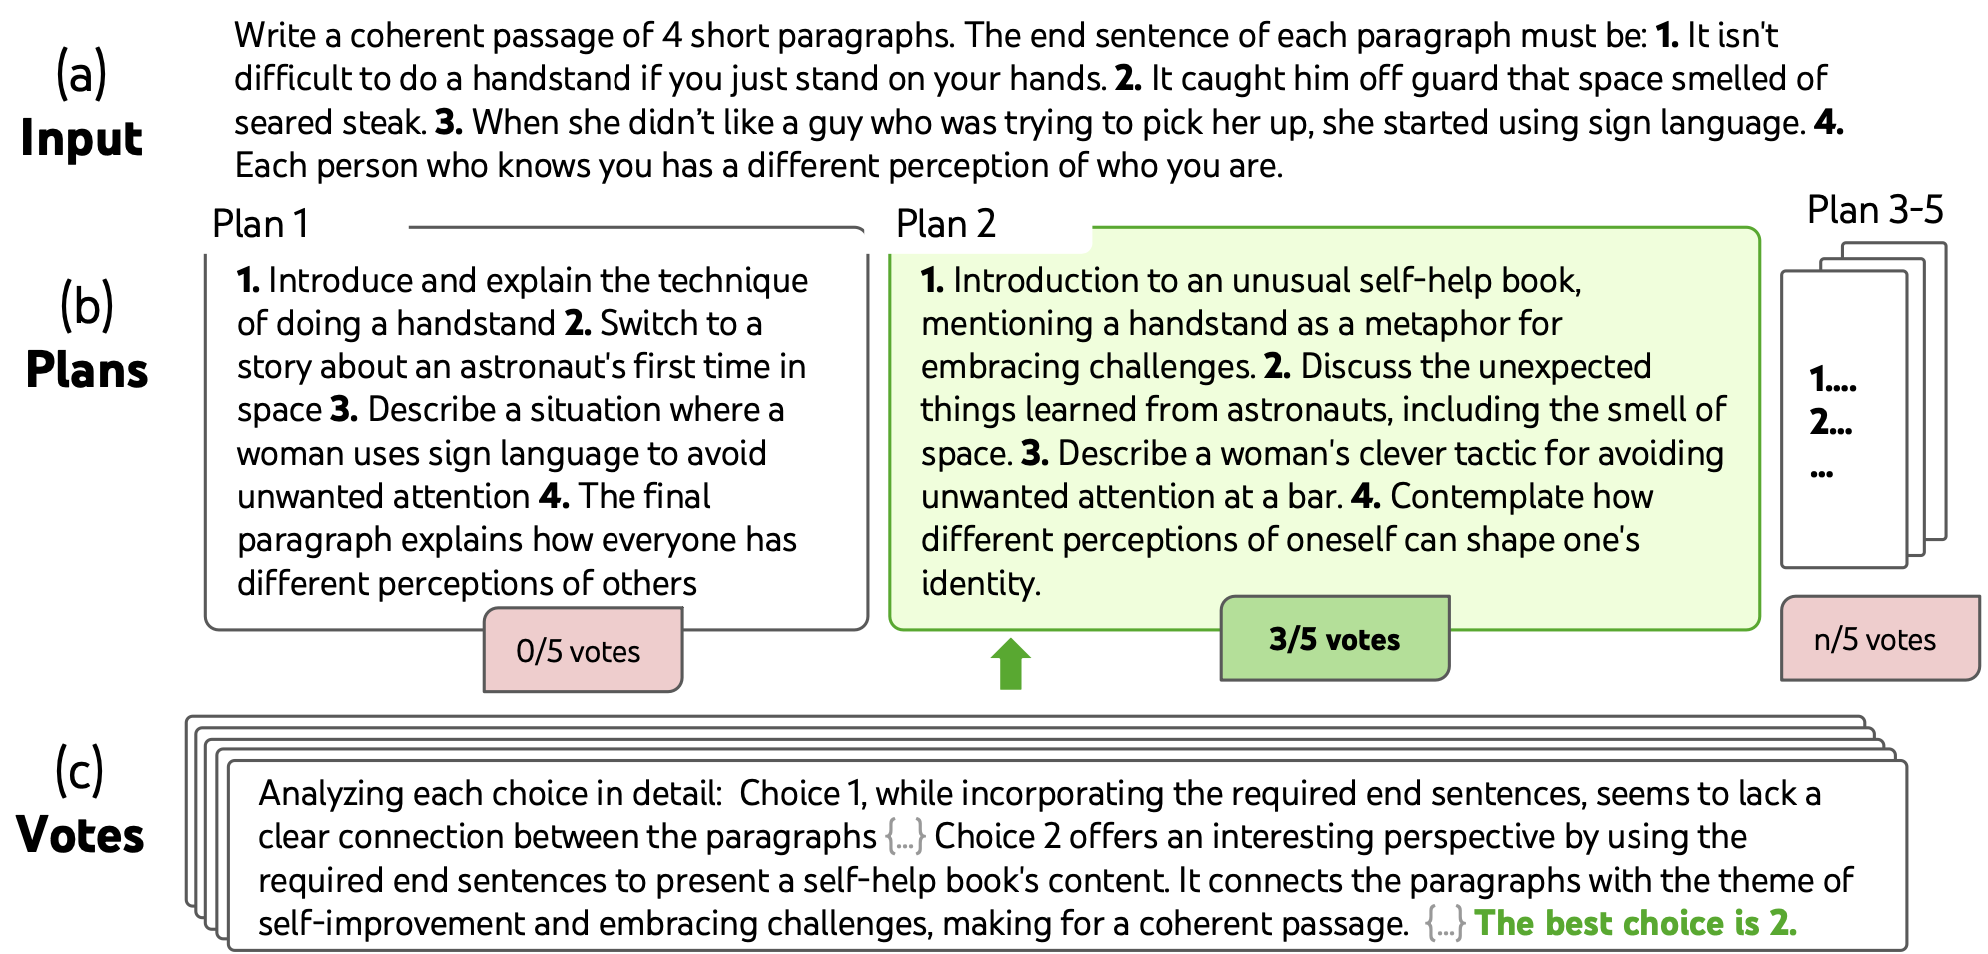
\includegraphics[width=1.15\textwidth]{figure/totcreativebig.png}}
\end{figure}

\vfill

\end{vbframe}

% ------------------------------------------------------------------------------

\endlecture
\end{document}
